\chapter{関連研究}
この章ではまず,既存のボードゲームAIについてAlphaZeroを中心に強化学習的枠組みからその理論を説明する.
次にAlphaZeroの問題点について述べ,
それを補完する既存手法,その課題について述べる.



\section{強化学習}
強化学習はタスクを選択をする主体と環境のやり取りとして定式化し,その相互作用から学習を行う形でタスクに取り組む分野である\cite{RL}.

強化学習タスクでは能動的に行動を行う主体と,主体が働きかける環境を設定する.図\ref{fig:RL}に示すように環境の状況は状態$s$として定義され,
$s$に対する主体の行動$a$によって環境の次の状態${s'}(=T(s, a), Tは遷移関数)$と主体が獲得する報酬$r$が決定されると仮定する.
その仮定の下,環境から主体に与えられる報酬の合計$G$($=\Sigma r$以下収益と記載)を最大化することを目標とする.
報酬を大きくするためには各状態$s$に応じて適切な(より大きな報酬をもらえる可能性が高い)行動を選択する必要がある.
\begin{figure}[t]
	\centering
	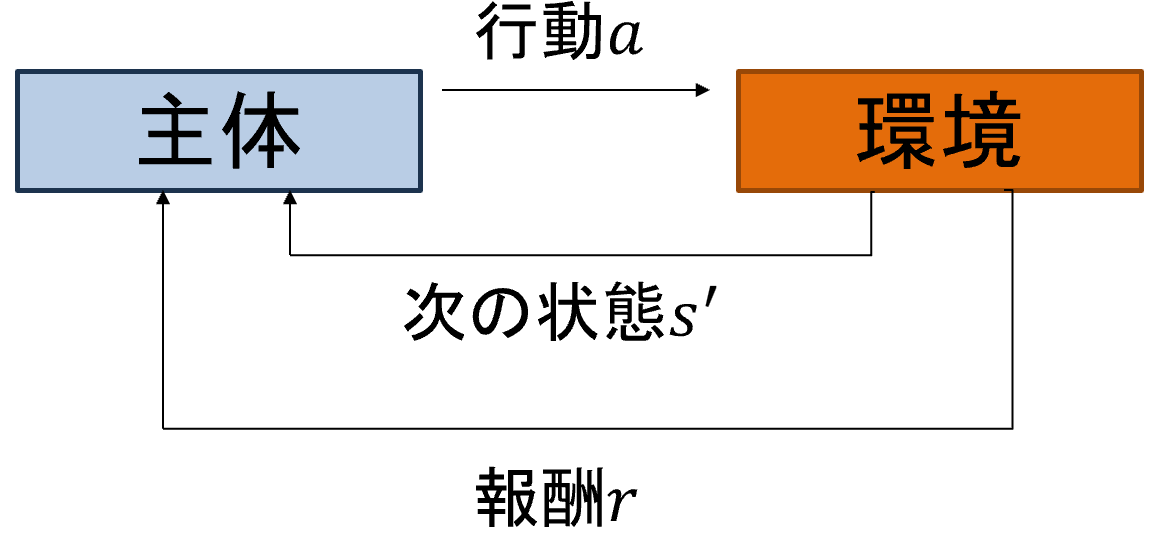
\includegraphics[width=\linewidth]{./figure/RL.png}
	\caption{強化学習}
	\label{fig:RL}
\end{figure}
そのため状態$s$に対して行動$a$をとった場合の収益に対して見積もりをとり,見込まれる値が最も大きい行動を選択することでより大きな収益を獲得できると期待できる.
このような収益の見積もりを$Q(s, a)$とした場合,
\begin{equation}
	{\displaystyle a_m = {\textrm{argmax}}_{a} Q(s, a)}
\end{equation}
となる$a_m$を選択することによって収益の最大化が期待される.また,状態$s$から獲得できる収益の合計の予想値$V(s)$(以下状態価値関数と表記)は,最適な行動$a_m$を取った場合の値として推定される.
\begin{equation}
	{\displaystyle V(s) = Q(s, a_m)(a_m = \textrm{argmax}_{a} Q(s, a))}
\end{equation}
強化学習手法によってタスクの最適化を図る際にはこの$V(s),Q(s, a)$を正しく推定することが直接的な目標となる.$V(s),Q(s, a)$は主体が実際に環境とやり取りを行う(タスクを実行していく)中で改善されていくことが期待される.
Temporary Difference法やMonte Carlo法等が基本的な$V(s),Q(s, a)$の更新則であり,DQN\cite{DQN}やRainbow\cite{rainbow}等はニューラルネットワークを使用して$V(s),Q(s, a)$
を推定することでより高い性能を発揮している.



\subsection{ボードゲームへの応用}
ボードゲームでは通例,状態$s$は盤面の状況,行動$a$はプレイヤーの選択,報酬$r$はゲームの最後に勝敗として与えられる.
図\ref{fig:board-game-model}に状態$s$(ゲームの状況)と行動$a$(プレイヤーの選択)によって盤面は次の状態$s'$に遷移し,次の行動$a'$(他のプレイヤーによる選択)を受け付ける,というサイクルとしてゲームの進行を定式化して表現することができる.
また,上述した強化学習における状態価値関数$V(s)$の推定は「ある盤面はプレイヤーにとって勝利に近いのか」を表現していると解釈され,行動価値関数$Q(s, a)$は「ある盤面である行動をした場合のプレイヤーの勝率」を表していると解釈される.
AlphaGo\cite{AlphaGo}やStockFish\cite{StockFish12},DeepLearningShogi\cite{dlshogi}では状態$s$は最新$N$ステップの盤面と手数などのゲームのプレイにおいて重要な情報である.
状態は行列等の形式に抽象化され,行動は次にプレイヤーが打つ箇所の座標となる.
\begin{figure}[t]
	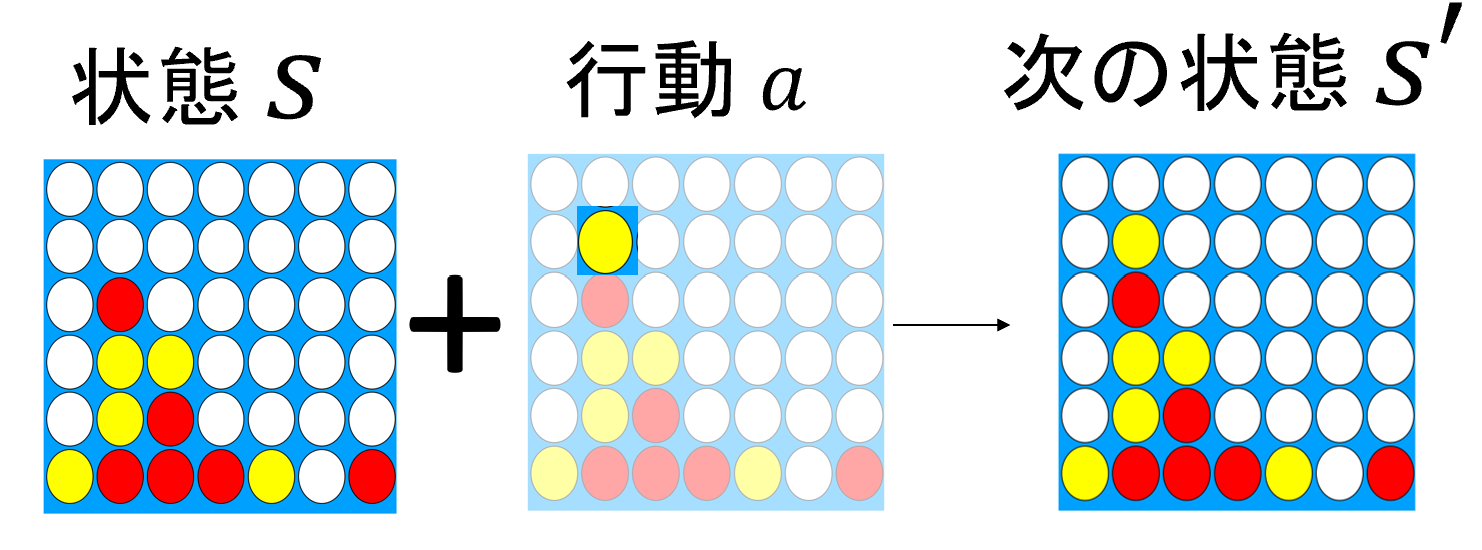
\includegraphics[width=\linewidth]{./figure/transition.png}
	\caption{ボードゲームにおける強化学習モデル}
	\label{fig:board-game-model}
\end{figure}

また,図\ref{fig:connect4-symbol}に示すように本論文で使用したalphazero\_baselineモデル\cite{baseline}における入力は最新の盤面の状態を空白を0,先番(赤)の石の位置を1,後番(黄)の位置を-1として抽象化した6$\times$7の行列となる.
\begin{figure}[t]
	\centering
	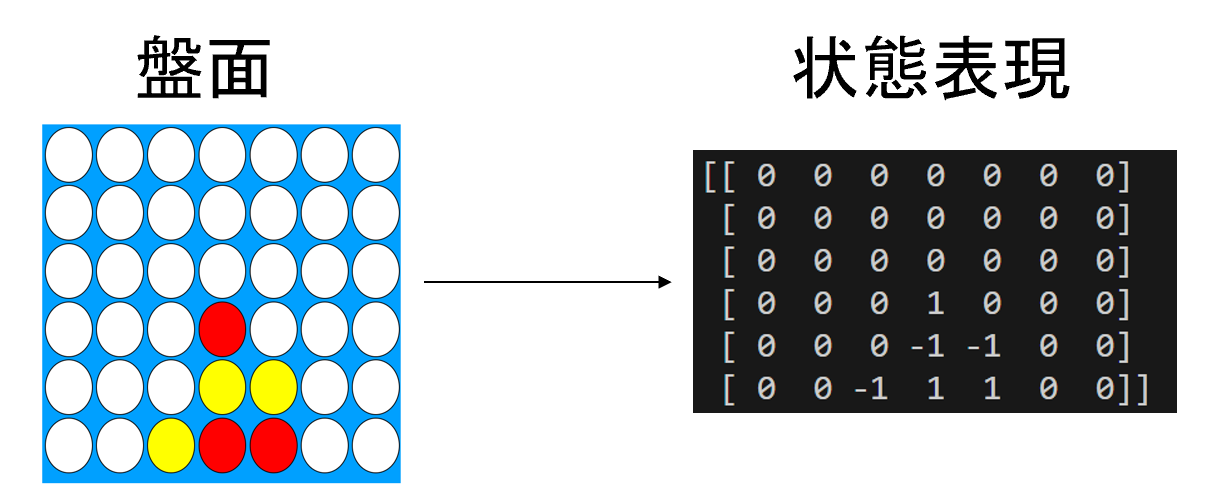
\includegraphics[width=\linewidth]{./figure/symbolic.png}
	\caption{connect4盤面の状態表現}
	\label{fig:connect4-symbol}
\end{figure}
また,後述するconnect4のルール上の制約により次にプレイヤーが打つ箇所(行動)は列の数と同数の7種類に限定される.

\subsection{AlphaZero}
AlphaZeroは2016年に登場し,囲碁の元世界チャンピオンであるイ・セドルに対して四勝一敗の成績を収めたAlphaGoの汎用版であり,囲碁・将棋・チェスなどの主要なボードゲームにおいて人間の実力を凌駕したパフォーマンスを誇る.
AlphaZeroは先述の$V(s),Q(s, a)$を推定する際にニューラルネットワークとPV-モンテカルロ木探索アルゴリズムを使用する.
\paragraph{ニューラルネットワーク}
AlphaZeroにおけるニューラルネットワークの構造を図\ref{fig:network}に示す.
AlphaZero内のニューラルネットワークに対する入力は最新$8$ステップの盤面($\left\{ s_{-7}, ..., s_0 \right\}$,$s_{-i}$は$i$ステップ前の盤面,$s_{0}$は現在の盤面)であり,出力は方策$P(\left\{ s_{-7}, ..., s_0 \right\})$と
局面評価$V(\left\{ s_{-7}, ..., s_0 \right\})$の二種類である.
ネットワークは1つの畳み込み層と20の残差結合ネットワークで構成されている.  \\
方策は「現在の状況から次にどこを選択すべきか」を表現しており,次に選択すべき座標を確率分布の形式で表現する.
方策内の値の大きさがAIによるその着手の評価と解釈され,成分が大きい座標を次に選択することが推奨される.\\
また,局面評価$V(\left\{ s_{-7}, ..., s_0 \right\})$は「(過去7ステップ分の情報を含めた)現在の状況$s_0$は勝利に近いのか」を表現しており,値が上限に近ければ近い程,現在の状況$s_0$が次の着手を選択するプレイヤーにとっての勝利に近いことを表している.
\begin{figure}[t]
	\centering
	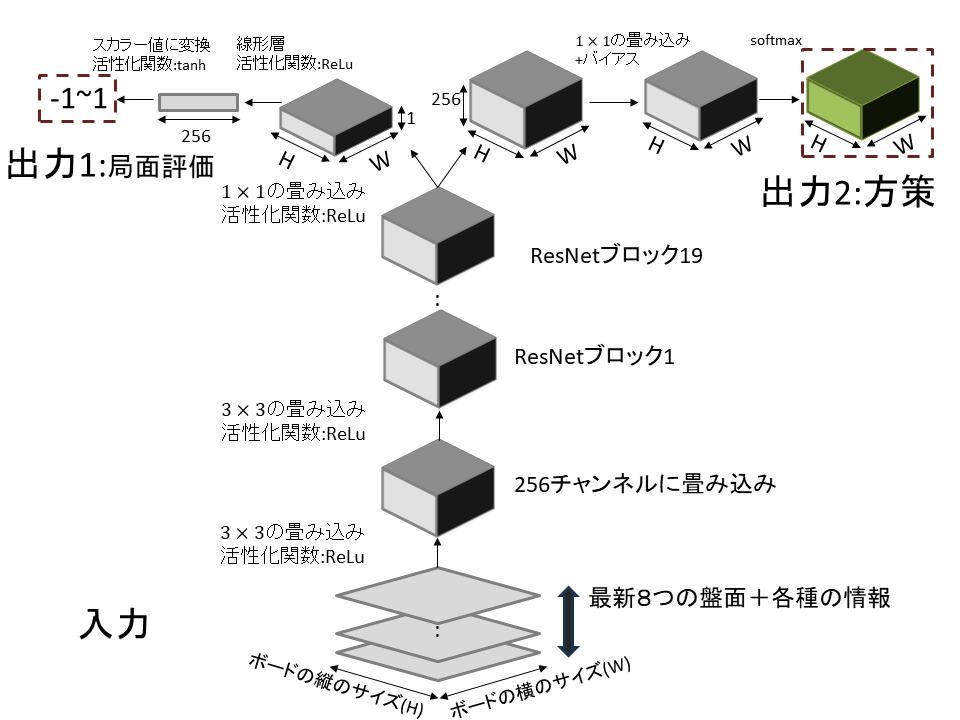
\includegraphics[width=\linewidth]{./figure/network.png}
	\caption{AlphaZeroネットワークの構造}
	\label{fig:network}
\end{figure}
\paragraph{PV-モンテカルロ木探索}
PV-モンテカルロ木探索ではニューラルネットワークから得た方策$P(s)(以下s=\left\{ s_{-N+1}, ..., s_0 \right\}と表記する)$と局面評価$V(s)$をシミュレーション
によって改善する.
PV-モンテカルロ木探索ではシミュレーションによって$s$または$(s, a)$(状態と行動の組)をノード,各行動$a$を枝とした決定木を構築する.
最終的に各ノード$s$から派生する各行動$\left\{a_1, a_2, ..., a_n\right\}$の探索回数の分布$N(s)(={N(s, a_1), N(s, a_2), ..., N(s, a_n)})$が改善された方策となる.
一方,局面評価もまたモンテカルロ木探索により決定木が拡張されるなかで更新される.Algorithm\ref{alg:mcts-1},Algorithm\ref{alg:mcts-2}に決定木と局面評価$V(s)$の詳細な更新アルゴリズムを示し,ここでは大まかな流れを示す.
PV-MCTSのアルゴリズムの流れは以下の通りである.
(余裕があれば図を追加)
\begin{enumerate}
    \item まず,探索の開始地点となるノード$s$を決定する.
    \item 再帰部分では以下の処理を再帰的に呼び出す.
    \begin{enumerate}
        \item ノード$s$を探索したことがない場合
        ニューラルネットワークから出力された方策$P(s)$と局面評価$V(s)$を返却する.
        \item ノード$s$を探索したことがある場合
        以下のpuctスコア$U(s, a)$と行動価値関数$Q(s, a)$の和が最大となる子ノード$s_c(=T(s, a))$を選び,$s_c$に対してさらに再帰的に探索を行いその結果である$P(s_e), V(s_e)(s_eは再帰処理の結果たどり着く
        決定木の端のノード)$を返却する.($N(s), N(s, a)はそれぞれs,(s, a)に対して探索を行った回数$)
        \begin{equation}
            {U(s, a)= C(s)P(s, a)\frac{\sqrt{N(s)}}{1+N(s, a)}\\
            }
        \end{equation}
        
        \begin{equation}
            {C(s)=\textrm{log}\frac{1+N(s)+C_{\textrm{base}}}{C_{\textrm{base}}}+C_{\textrm{init}}\\
            (C_{\textrm{base}}, C_{\textrm{init}}はハイパーパラメータ)}
        \end{equation}
    \end{enumerate}
\end{enumerate}


	
このようなプロセスによって決定木を構築しつつ,モデルは対戦を行う.
\newpage
\begin{algorithm}
    \caption{PV-MCTS in AlphaZero (Part 1: Exploration)}
    \label{alg:mcts-1}
    \begin{algorithmic}[1]
        \State $t$: 決定木
        \State $T$: 遷移関数
        \State $N(s, a)$: $(s, a)$の組み合わせを探索した回数
        \State $Q(s, a)$: 行動価値関数 
        \State $W(s, a)$: 行動価値の総和$(W(s, a)=Q(s, a)N(s, a))$
        \State $P(s, a)(=P(s_n), s_n=T(s, a))$: 
        \State ニューラルネットワークから出力された方策
        \State $V(s, a)(=V(s_n), s_n=T(s, a))$: 
        \State ニューラルネットワークから出力された局面評価
        \Function{Explore}{$s_{\text{start}}$}
            \State Set $s_{now} = s_{start}$ and $a_{now} = a_m$
            \For {each simulation}
                \State $\zeta \gets \textrm{empty list}$
                \State $s_{\text{current}} \gets s_{\text{start}}$
                \While {$s_{\text{current}}$ がゲームの終了状態でない場合}
                    \State $a_t \gets TreePolicy(s)$
                    \State (Tは遷移関数)
                    \State $(s_{\text{current}}, a_t)$を $\zeta $の末尾に追加
                    \State $s_{\text{next}} \gets T(s_{\text{current}}, a_t)$
                    \State $s_{\text{current}} \gets s_{\text{next}}$
                    
                \EndWhile
                \State $G \gets V(s_e)$ 
                \State($s_e$は$s_{start}$から探索してたどり着いたノード$s_e$)
                \State \Call{Backpropagate}{$\zeta, G$}
            \EndFor
        \EndFunction
        
        
    \end{algorithmic}
\end{algorithm}
\begin{algorithm}
    \caption{PV-MCTS in AlphaZero (Part 2: Backpropagation)}
    \label{alg:mcts-2}
    \begin{algorithmic}[1]
        \Function{TreePolicy}{$s$}
            \If {$s$が探索されていない子ノードを持つとき}
                \State $s_c \gets T(s, a)$ ($s_c$は未探索のノード)
                \State \Call{InitNode}{$s_c$}
                \State \Return $a$
            \Else
                \State 以下のPUCTスコア$U(s, a)$を計算
                \State $U(s, a)= C(s)P(s, a)\frac{\sqrt{N(s)}}{1+N(s, a)}$
                \State $C(s)=\textrm{log}\frac{1+N(s)+C_{\textrm{base}}}{C_{\textrm{base}}}+C_{\textrm{init}}$
                \State($C_{\textrm{base}}$, $C_{\textrm{init}}$はハイパーパラメータ)
                \State $(N(s)=\Gamma N(s, a))$
                \State 以下のように$a$を求める
                \State $a = {\textrm{argmax}}_a (Q(s, a)+U(s, a))$
                \State \Return $a$
                
            \EndIf
        \EndFunction
        \Function{Backpropagate}{$\zeta, G$}
            \For {each node-action pair $(s, a)$ in $\zeta$}
                \State $N(s, a) \gets  N(s, a)+1$
                \State $W(s, a) \gets  W(s, a)+G$
                \State $Q(s, a) \gets \frac{W(s, a)}{N(s, a)}$
            \EndFor
        \EndFunction
        \Function{InitNode}{$s$}
            \For {each action $a$ from  $s$}
                \State $N(s, a) \gets 0$
                \State $W(s, a) \gets 0$
                \State $Q(s, a) \gets 0$
            \EndFor
        \EndFunction
    \end{algorithmic}
\end{algorithm}


\subsection{ボードゲームAIの問題点}
AlphaZeroは当時の正解最高峰のAIであるチェスのStockFish\cite{StockFish}や将棋のelmo\cite{elmo}を凌ぐ性能を発揮した.
それらの従来の有力なボードゲームAIは設計がそのゲーム固有の知識(ドメイン知識)に依存する割合が多かったため,
「ある条件を満たすときにある選択をする」と言ったようにその挙動をルールの集合として解釈できる余地があった.その意味ではStockFIsh12やelmoはその設計が説明性を有していたといえる.
一方で,AlphaZeroのニューラルネットワークと木探索を組み合わせた手法では方策と局面評価の根拠を得ることができない.つまりAlphaZeroの問題点として説明性の欠如が挙げられるのである.
2024年現在,StockFish・elmoの両者も人間の知識データへの依存を減じる方向に改良を続けており,性能と設計の説明性がトレードオフ関係にあると言える\cite{elmo}\cite{StockFish13}.
説明性の欠如はAIの判断に対する責任の不在を意味し,システムのよりハイレベル,ハイリスクなタスクへの実用化に対する妨げとなっている.
そのため,設計段階では説明性を持たないシステムに対して説明性を付加する手法を構築する必要がある.




\section{XAI}

\subsection{概要}
XAIとはExplainable AI(説明可能AI)の略語であり,AIモデルの結果を説明し,理由付けを行う際のシステムとユーザーのコミュニケーションに焦点当てた分野である\cite{consider}.
本研究はAIの判断根拠として先読みを示す面でXAIの分野に属する研究であると言える.
ここでの「説明可能性」の語は「人間に理解できる形での説明を与える能力」\cite{definition}と定義され,
\begin{itemize}
    \item いつ
    \item どのような
    \item どのように
\end{itemize}
説明を与えるかによってさらに細かく分類される.\\
「いつ」,つまりどの時点で説明を与えるかに関しては既存のネットワークに対して新たに説明を加える「事後的」説明と初めから動作の根拠を示せるようにネットワークやシステムを構築する「事前的」説明
に分類できる\cite{definition}.\\
「どのような」,つまり説明の内容については「大域的」説明と「局所的」説明の二つに分類される.「大域的」説明は行動$a$を選択する主体(モデル)の全体的な方針について述べるものである一方で,「局所的」説明は主体(モデル)の個々の判断について説明する\cite{gl}.
また,「どのように」,つまり説明を表現する形態としてはsaliency map\cite{saliency}, Grad-CAM\cite{Grad-CAM}といった視覚的な可視化や,教師データと予測結果との因果関係の数値的な定量化\cite{定量},入力の出力への寄与を表すグラフや説明文の生成\cite{LIME}
が挙げられる.\\
本論文において構築するシステムは「事後的」「局所的」「視覚的」説明を提供する.

また,本論文はXAI分野の中でも特に強化学習方面に対して説明を加える領域をXRL(Explainable Reinforcement learning)と呼ぶ.(余裕があったら追加,XRLの試みは様々な強化学習システムを対象とし,)
\subsection{ゲームにおけるXAI}
McGrathら\cite{DeepMind}はチェスにおける人間の知識や理論がAlphaZeroにどれだけ反映されているかを訓練段階やネットワークの深さなどの多様な指標で調査した.
他にも,Leeら\cite{DecodeChess}によるAIの着手に対してゲームの固有の知識(ドメイン知識)を用いたモデルの挙動に対する解説文の自動生成の試み等が存在する.
しかし,このようなドメイン知識は必ずしもAIの挙動と相関が無いことも指摘されている\cite{DeepMind}.
AIによる画像分類タスクの可視化手法として用いられていたsaliency map\cite{saliency}やGrad\_CAM\cite{Grad-CAM}を強化学習に用いる例も存在する\cite{gl}\cite{atari-saliency}\cite{visualize}.しかしそれらのニューラルネットワークの活性を根拠とした指標は木探索部分との繋がりが弱く,最終的に決定木を用いて意思決定を行うシステムの動作根拠を直接的に説明できない.
また,これらの画像分類用の手法は
\begin{itemize}
	\item 本来ゲームに存在する時系列の要素を説明に含められない
	\item 時系列を無視してゲーム画面や盤面の一部を変更する必要がある
\end{itemize}
という問題点が存在する.また,saliency mapやGrad-CAMは主にニューラルネットワークに対する説明手法であり,決定木への応用が困難さも欠点として挙げられる.

\subsection{contrastive explanation}
上述の問題点を解決するために,本論文の第4章におけるシステムではAlphaZeroが構築する決定木を用いたcontrastive explanation(対象説明,比較説明)を提供する.
contrastive explanationは事象を説明する際の方法論の1つであり,図\ref{fig:contrastive}に示すように
ある事象$a$が起こった際にその理由を直接説明する代わりに「他の事象$\bar{a}$が起こらなかった理由」を説明することで間接的にある事象$a$の原因を説明するアイデアである\cite{contrastive}.
Jacoviらの\cite{contrastive}では自然言語処理の分類タスクにおいて本来の入力データと編集された入力データの出力を比較することで,入力のどの部分がモデルの判断に寄与しているかを示している.
Mishraらの\cite{whyNot}では医療タスクにおけるニューラルネットワークの判断を決定木に近似した上でAIの判断$a$から派生する予想と別の判断$b$から派生する予想を提示する形でAIによる判断の妥当性を示している.
また,Gajcinらの\cite{preference}では異なるモデルの挙動の違いをユーザーに示す目的でcontrastive explanationが用いられている.
これらの強化学習・木構造ネットワークに対するconstrative explanationの手法は決定木上の「最も可能性が高い」「単一の」予想図を用いることを前提としている.
そのため第3章でしめす提案手法では決定木上の複数の予想図を用いたconstrative explanationの実現を試みた.

\begin{figure}[t]
	\centering
	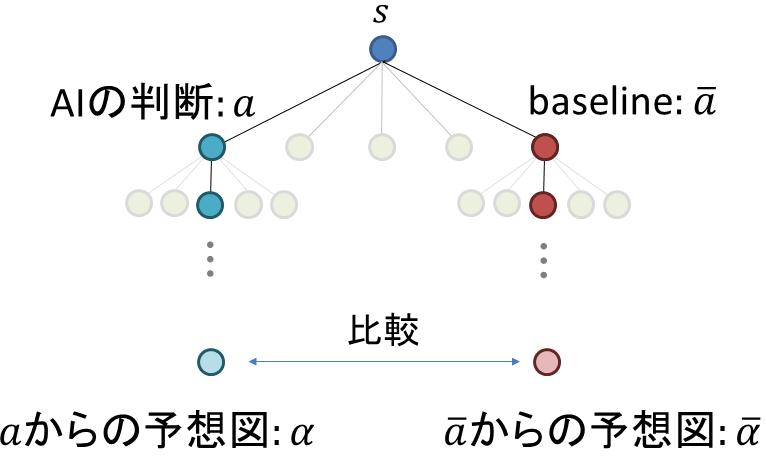
\includegraphics[width=\linewidth]{./figure/contrastive.png}
	\caption{contrastive explanation}
	\label{fig:contrastive}
\end{figure}
\subsection{importance}
ゲームやタスクにおいて勝負の分かれ目となりうる場面や,ミスをしやすい場面,危険な事故が起きやすい場面を特定することは非常に有用である.また,このようなAIモデルが他の場面よりも重要度が高いと判断する状況を収集することは,モデルの挙動に対する効率的な調査を可能にする.
Torrayら\cite{imp2013}やAmirら\cite{imp2016}は状態の重要度$I(s)$を一つ先の行動価値関数$Q(s, a)$が次の選択によって大きく左右されるような状態を重要度の高い局面として定義している.
$Q(s, a)$の揺らぎの捉え方にはいくつかの方式が存在し,
Torrayらは$I(s)$を$s$から辿り着きうる最善の$Q(s, a)$と最悪の$Q(s, a)$の差として定義している.
\begin{equation}
	{I(s)= \textrm{max}Q(s, a)-\textrm{worst}Q(s, a)}
\end{equation}
Amirらは$I(s)$を$s$から辿り着きうる最善の$Q(s, a)$と二番目に値の大きい$Q(s, a)$の差として定義している.
\begin{equation}
    \label{imp}
	{I(s)= \textrm{max}Q(s, a)-\textrm{secondMax}Q(s, a)}
\end{equation}
しかし,これらの定義はimpが$Q(s, a)$の値が低くなるような行動$a$に大きく影響されるリスクや,図\ref{fig:symmetry}のように状態に対称性があるような場合に重要度が過度に小さくなってしまうリスクがある.
\begin{figure}[t]
	\centering
	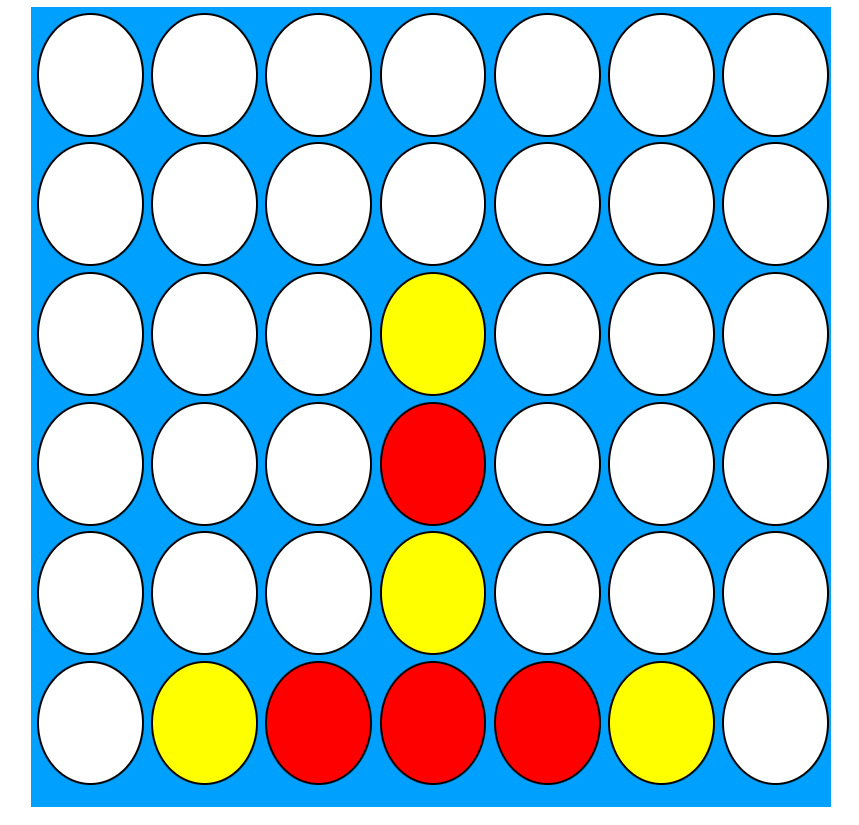
\includegraphics[width=80pt]{./figure/symmetry.png}
	\caption{対称性がある盤面の例}
	\label{fig:symmetry}
\end{figure}
また,Guoら\cite{EDGE}は重要度$I$を収益$G$が確定するまでの一連の流れ(エピソード)やエピソード内の時点$t$の重要度を収益$G$との関連度の大きさから多角的に定めている.
しかし,Guoらの定義は状態の符号化や回帰などのデータの加工段階が多く,指標自体の説明性に疑問が残る.AIモデルに対して説明を加える際にはその手法自体もなるべく簡明であり,勝敗に直結している方が望ましいと考えられる.





\subsection{ボードゲーム学習支援}
本論文は高度なAIの動作を人間に理解させることを目標としており,学習支援の側面を含んでいると言える.
既存のAIを用いたボードゲーム学習支援システムとしてはLeeら\cite{ChessComments}やオンラインサービスであるDecodeChess\cite{DecodeChess}などによる解説文自動生成や,Richard\cite{badMoves2016}らやRichard\cite{badMoves2017}らの人間側の悪手を自動的に検知しその理由を個別に指摘するモデルが提案されている.
しかし「ボードゲームに対するXAI」の段での内容と同様にゲームのドメイン知識に依存しており,指導の内容も人間の知識に依存したものになってしまうという欠点がある.
また,指導に特化した人間が挙動に違和感を抱きづらいAIの開発も行われている\cite{natural}\cite{maia}.
このアプローチは人間が受け入れやすい方向にAIの側を変更する方式であり,その変更により既存の人間の知識ではとらえられないAIの強みが失われてしまう危険性がある.


